\documentclass{article}
\usepackage{graphicx}  % To include the visualization image
\usepackage{hyperref}  % For hyperlinks
\usepackage{geometry}  % For adjusting margins
\geometry{a4paper, margin=1in}

\title{FIT3179 Week 9 Homework Report}
\author{Your Name}
\date{\today}

\begin{document}

\maketitle

\section*{Introduction}
This report presents a proportional symbol map visualizing the public transport ridership in Malaysia. The map highlights the daily ridership across various locations in Malaysia using circles with varying sizes based on ridership values. The map was generated using Vega-Lite, and the data was cleaned and sourced from public ridership datasets.

\section*{Data Description}
The data used for this visualization was a cleaned CSV dataset containing information on public transport ridership across different regions in Malaysia. The dataset includes key columns such as:
\begin{itemize}
    \item \textbf{Location:} Name of the transport hub or city.
    \item \textbf{Latitude:} Latitude coordinates for the location.
    \item \textbf{Longitude:} Longitude coordinates for the location.
    \item \textbf{Ridership:} Daily ridership numbers.
\end{itemize}

The dataset was pre-processed to remove any null or zero values in the ridership column, ensuring the accuracy of the proportional symbol map.

\section*{Visualization Design}
The proportional symbol map employs an \textbf{equirectangular projection}, centered on Malaysia. Each circle on the map represents a public transport hub, and its size is proportional to the ridership data. A graticule layer was added to improve geographical orientation. The map includes the following layers:
\begin{itemize}
    \item \textbf{Base Map:} Malaysia’s boundaries were visualized using a TopoJSON file from public datasets.
    \item \textbf{Proportional Symbols:} Circles representing ridership values. Larger circles indicate higher ridership, with the circle size scaled between 0 and 100,000.
    \item \textbf{Graticule:} A grid of latitude and longitude lines to aid map readability.
\end{itemize}

\begin{figure}[h!]
    \centering
    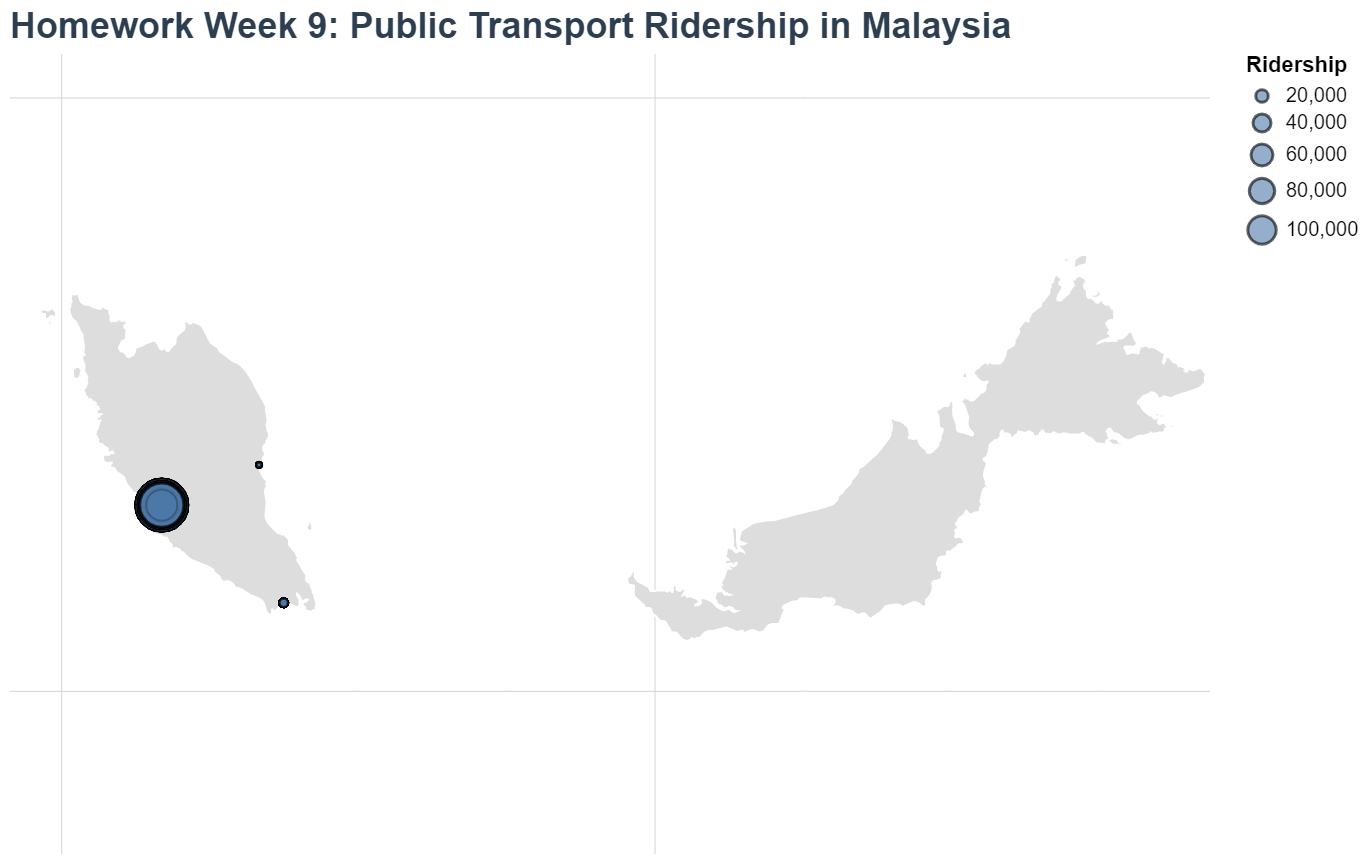
\includegraphics[width=\textwidth]{week9hwvisualization.png}
    \caption{Proportional symbol map showing public transport ridership in Malaysia.}
\end{figure}

\section*{Map Justification}
A proportional symbol map was chosen for this task because it provides a clear and intuitive way to compare ridership levels across various locations in Malaysia. This method allows for immediate visual comparison of the size and relative importance of each transport hub based on its ridership data.

The map design ensures clarity, with circle sizes directly proportional to ridership values and a tooltip providing detailed information for each hub. The graticule adds a layer of geographic context, ensuring the map remains easy to interpret.

\section*{Conclusion}
This map effectively visualizes the daily ridership of public transport hubs in Malaysia, providing an insightful way to compare ridership across different locations. By using a proportional symbol map and overlaying it on a detailed boundary map, this visualization clearly conveys both geographic and data-driven insights.

\section*{Links}
You can view the interactive version of this map on \href{https://your-github-page-link-here}{GitHub Pages}.

\end{document}
